\section{Department of Computer Science Ethics Checklist}
\renewcommand{\labelenumi}{\arabic{enumi})}

\begin{center} UNIVERSITY OF BATH \\[0.3cm] \textbf{Date:} 16/03/17 \end{center}

This document describes the 13 issues that need to be considered carefully before students or staff involve other people (``participants'') for the collection of information as part of their project or research.

\begin{enumerate}[Q.1]
	\item\textbf{Have you prepared a briefing script for volunteers?} \par
	\textit{The introductory script reads as follows:} \par ``As part of my dissertation on reducing news overload, I'm conducting a research study into how young people respond to different news presentation formats. \par I have a brief survey and consent form which should take about two minutes to complete.  The study consists of three questions related to your news habits, then fifteen minutes spent exploring some news content using two different interfaces and answering questions on those. \par In total, the study should take around twenty minutes. During the study, your voice will be recorded. Afterwards, the recording will be anonymously named and securely stored. No other personally identifying information is being collected. \par Your participation in this study is completely voluntary, you may skip any questions that you don't want to answer, or withdraw at any point. \par Thank you for your participation. Do you have any questions?''
	\item\textbf{Will the participants be using any non-standard hardware?} \par
	The study does not involve the use of any non-standard hardware.
	\item\textbf{Is there any intentional deception of the participants?} \par
	The study does not involve any deception of participants.
	\item\textbf{How will participants voluntarily give consent?} \par
	Participants will be asked to sign a consent form (See Appendix \ref{sec:consent}) and will be able to withdraw at any time during or after the study. 
	\item\textbf{Will the participants be exposed to any risks greater than those encountered in their normal work life?} \par
	The study does not involve any exposure to risk.
	\item\textbf{Are you offering any incentive to the participants?} \par
	No incentive will be offered to participants.
	\item\textbf{Are any of your participants under the age of 16?} \par
	All participants will be over the age of 18 so none will require parental consent.
	\item\textbf{Do any of your participants have an impairment that will limit their understanding or communication?} \par
	This study requires that all participants have perfect or corrected to perfect vision and hearing. Subjects with other communication impairments will not be eligible to participate in the study.
	\item\textbf{Are you in a position of authority or influence over any of your participants?} \par
	No, nor have I ever been.
	\item\textbf{Will the participants be informed that they could withdraw at any time?} \par
	The introductory script informs participants of this.
	\item\textbf{Will the participants be informed of your contact details?} \par
	All participants will be given my contact details before the study.
	\item\textbf{Will participants be de-briefed?} \par
	\textit{The debriefing script reads as follows:}
	``This study was conducted in order to evaluate people's understanding of news articles when they were presented in a graphically structured manner, versus a traditional list format. I want to test the hypothesis that news consumers feel less overloaded when given an overview of the news in the form of a metro map. \par I anticipate that overall, subjects will have identified a broader and longer list of topics in the index task and answered more optimistically in the guessing task using the metro map visualisation as opposed to the list view. I also anticipate that most subjects will use the connections in the map visualisation to help them answer the ``most important article'' question. \par Again, if you wish to contact me in future then you can email me at dtstb20@bath.ac.uk. Thanks for your time.''
	\item\textbf{Will the data collected from the participants be stored in an anonymous form?} \par
	Participants will be recorded using a dictaphone. Each audio recording will be kept with a numerical identifier for each participant, and recordings will be stored digitally with password-protection. No other personally identifying information will be collected.
\end{enumerate}

\section{User Study Consent Form}
\label{sec:consent}

Before the study, all participants were asked to read and sign the following consent form, which is based on an example from the University of Nottingham School of Education\footnote{\url{http://www.nottingham.ac.uk/educationstudentintranet/researchethics}}. \\[0.5cm]

\begin{center} PARTICIPANT CONSENT FORM \\[0.3cm] Newsfeed Visualisation with Metro Maps \end{center}

\textbf{Researcher:} Damask Talary-Brown (dtstb20@bath.ac.uk) \\
\textbf{Supervisor:} Professor Stephen Payne

\begin{enumerate}[1)]
\item The nature and purpose of the study has been explained to me and I agree to participate.

\item I understand the purpose of the research project and my involvement in it.

\item I understand that I may withdraw from the study at any stage and that this will not affect my status now or in the future.

\item I understand that while information gained during the study may be published, I will not be identified and my personal results will remain confidential.

\item I understand that my voice will be recorded during the interview and consent to this.

\item I understand that data will be stored securely and anonymously, where only myself and my supervisor have access to it.

\item I understand that I may contact the researcher or supervisor if I have any further questions or if I wish to make a complaint relating to my involvement in the research.\\[0.5cm]
\end{enumerate}

Participant Name: \dotfill \\[1cm]
Signed: \dotfill \hspace{0.5cm} Date: \dotfill 

\vfill
\section{User Study Metro Maps} \label{sec:evalmaps}
Both evaluation corpora were extracted from The Guardian's US News RSS Feed in March 2017. The station labelled $(a)$ in each map is the article expanded in the right hand pane.

\begin{landscape}
\begin{figure}[htbp!]
	\centering
	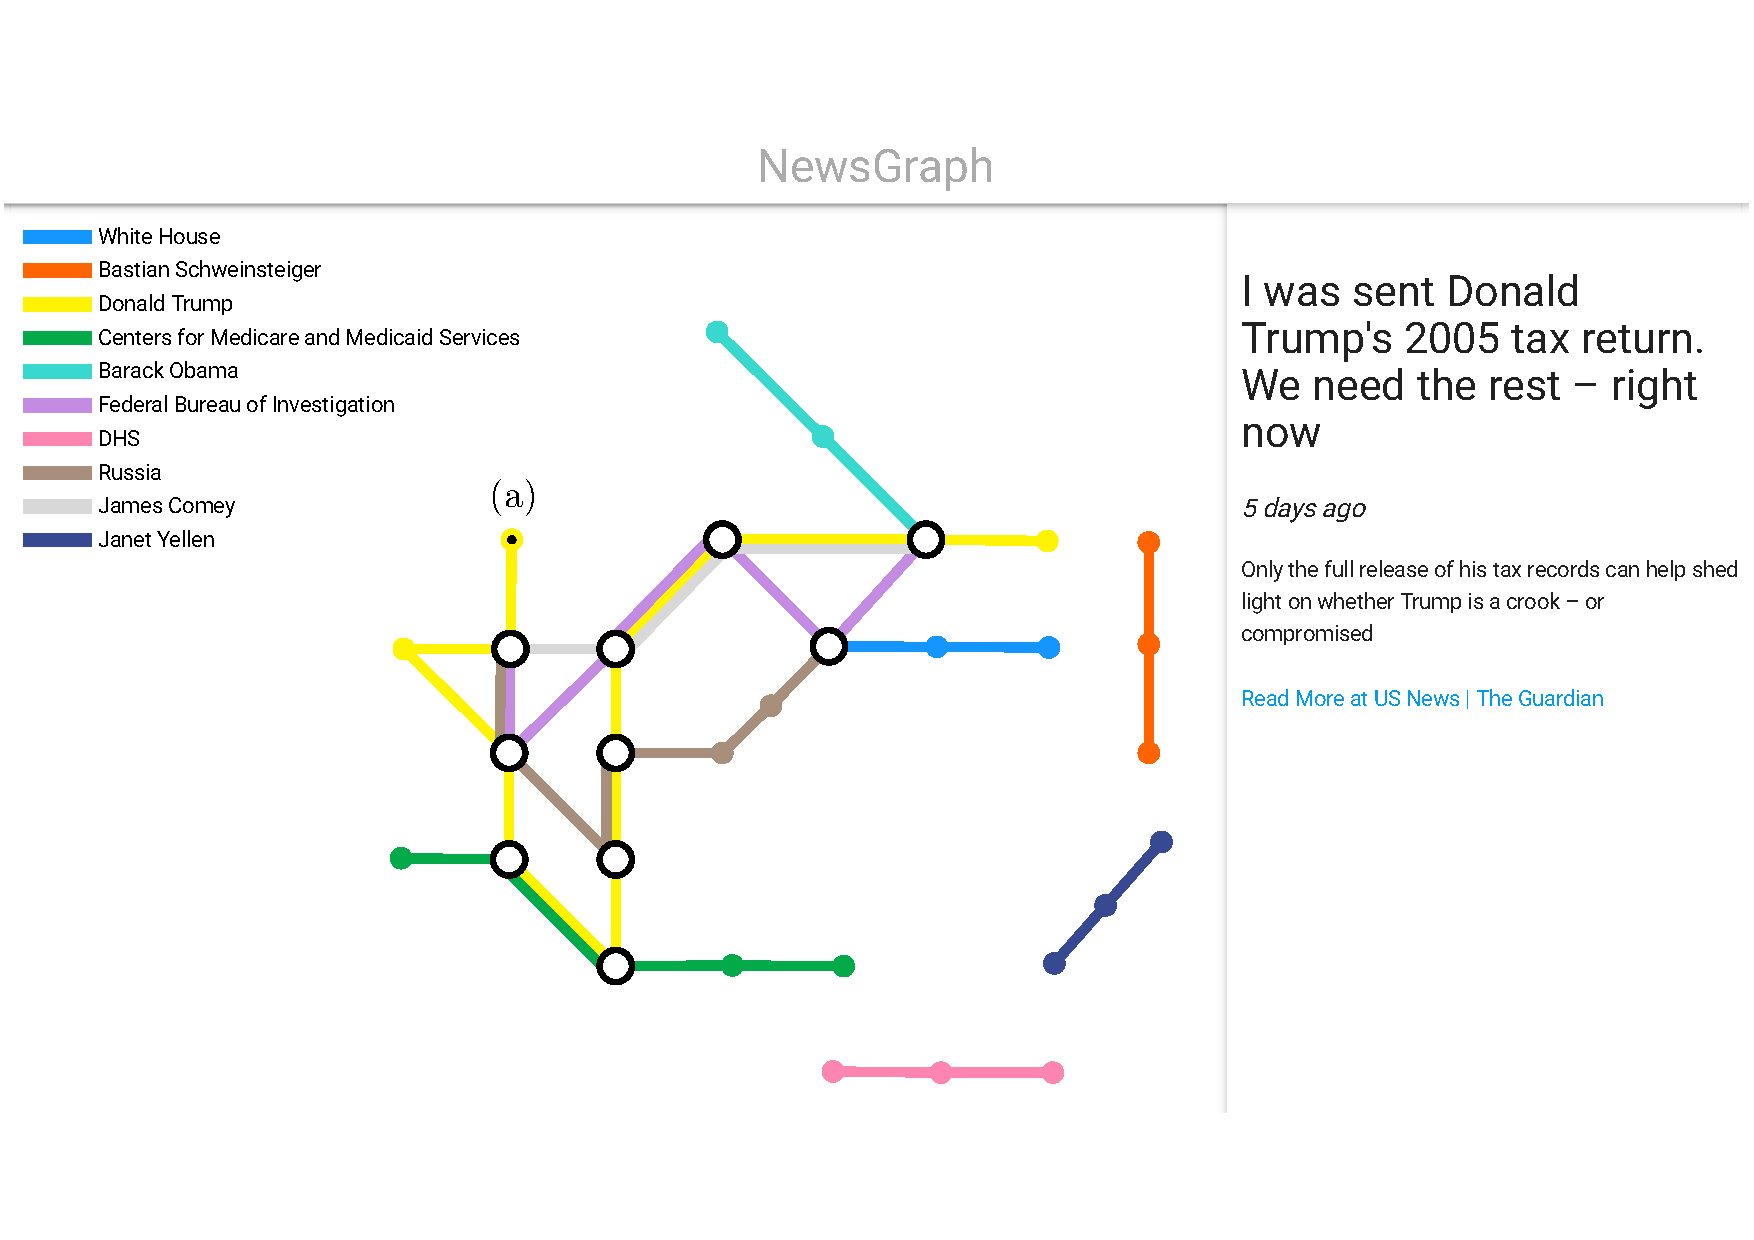
\includegraphics[width=1.3\textwidth]{img/evaluation/map1.pdf}
	\caption{User Study Data: Map A}
	\label{fig:map1}
\end{figure}
\end{landscape}
\begin{landscape}
\begin{figure}[htbp!]
	\centering
	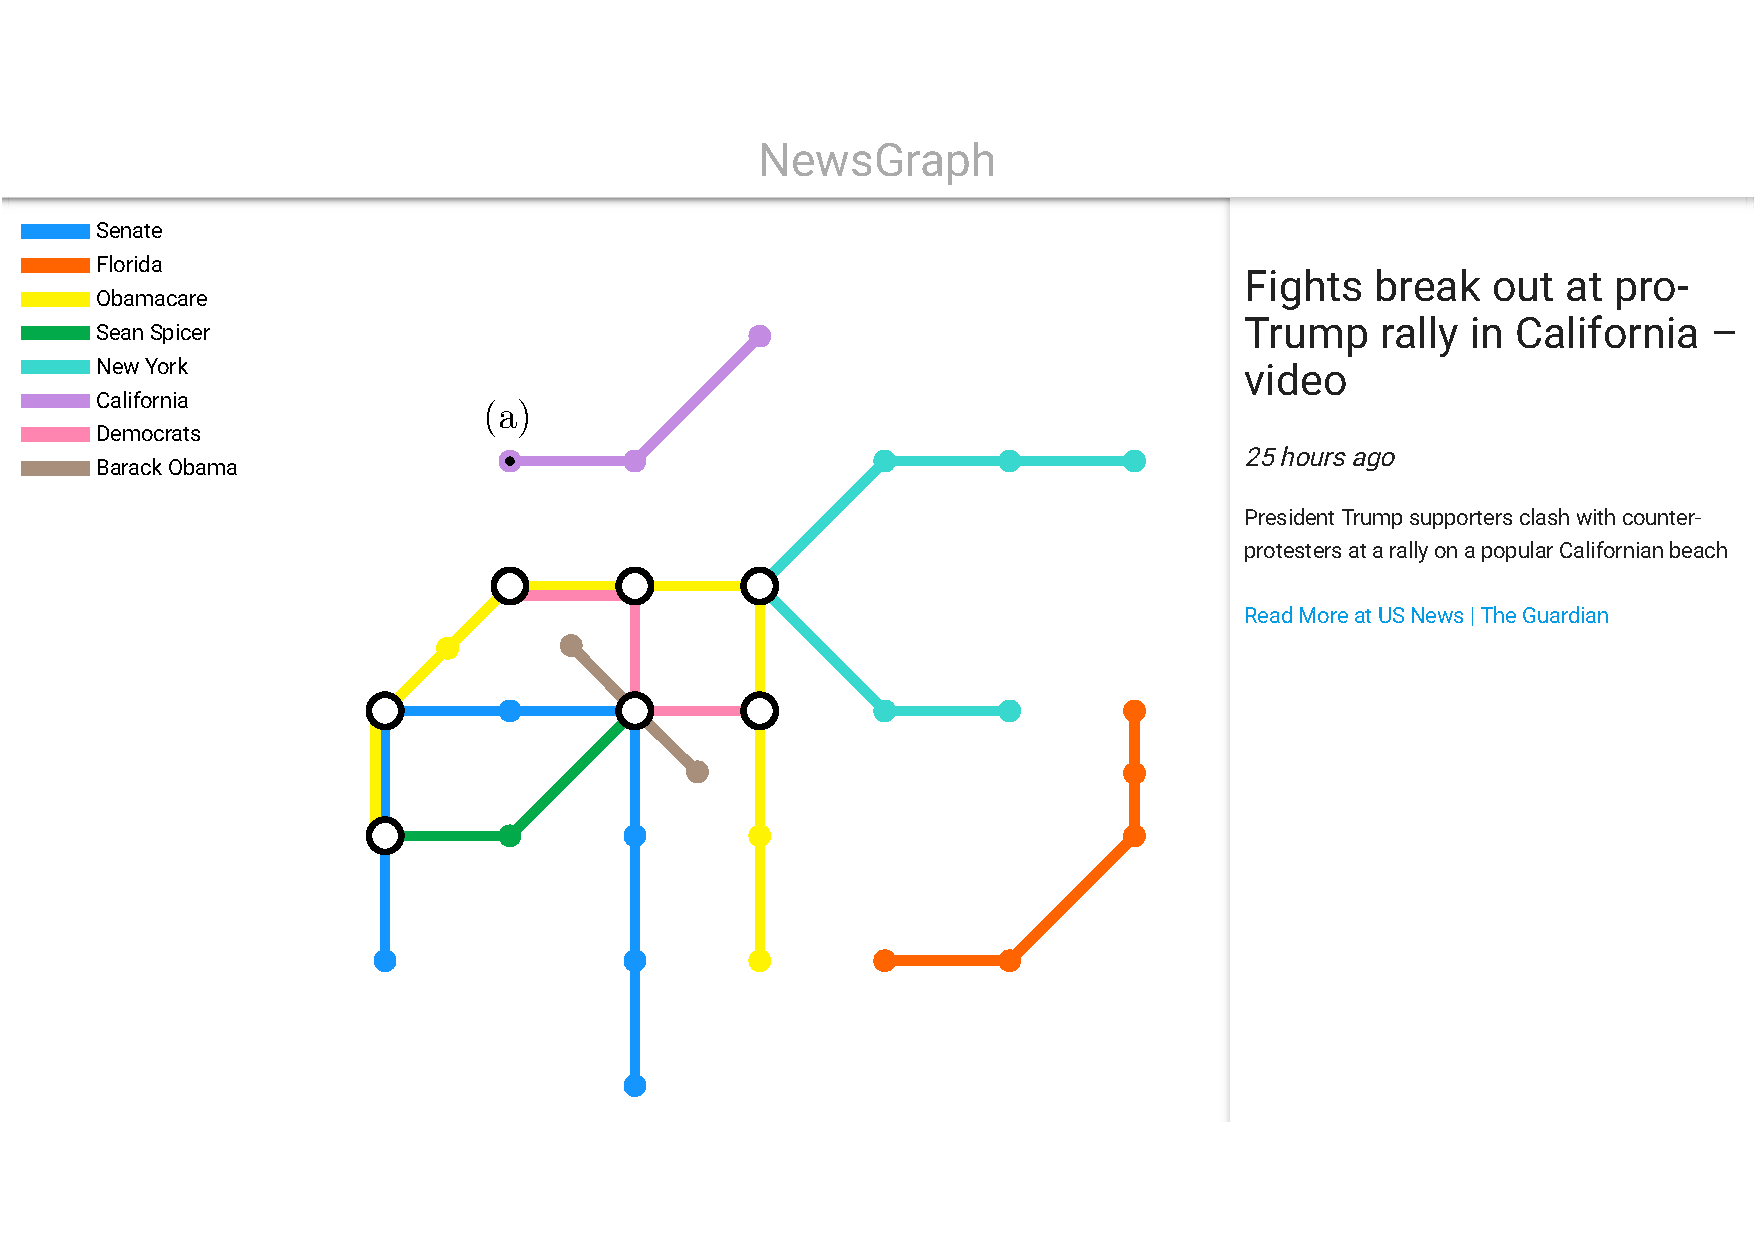
\includegraphics[width=1.3\textwidth]{img/evaluation/map2.pdf}
	\caption{User Study Data: Map B}
	\label{fig:map2}
\end{figure}  
\end{landscape}
\clearpage


\section{Evaluation Results} \label{sec:evalresults}

\begin{table}[hbtp!]
\centering
\caption{Means of \textit{Map Estimate} and \textit{List Estimate}} \vspace{0.3cm}
\label{res:estimatepre}
\begin{tabular}{|l|l|llll|}
\hline
\multicolumn{2}{|c|}{}  & Mean  & N  & Std. Deviation & Std. Error Mean \\ \hline\hline
\multirow{2}{*}{Pair 1} & Map Estimate  & 24.75 & 16 & 7.188          & 1.797           \\ \cline{2-6}
                        & List Estimate & 25.88 & 16 & 6.820          & 1.705
                        \\ \hline          
\end{tabular}
\end{table}

\begin{table}[hbtp!]
\centering
\caption{Means of \textit{Map Total Topics, Primary Topics, Depth} and \textit{List Total Topics, Primary Topics, Depth}} \vspace{0.3cm}
\label{res:indexpre}
\begin{tabular}{|l|l|llll|}
\hline
\multicolumn{2}{|c|}{}  & Mean  & N  & Std. Deviation & Std. Error Mean \\ \hline\hline
\multirow{2}{*}{Pair 1} & Map Total  & 10.94 & 16 & 4.389 & 1.097 \\ \cline{2-6}
                        & List Total & 8.88  & 16 & 2.156 & .539  \\ \hline
\multirow{2}{*}{Pair 2} & Map Primary  & 4.19  & 16 & 1.601 & .400  \\ \cline{2-6}
                        & List Primary & 3.25  & 16 & 1.125 & .281  \\ \hline
\multirow{2}{*}{Pair 3} & Map Depth  & 2.25  & 16 & .577  & .144  \\ \cline{2-6}
                        & List Depth & 2.31  & 16 & .602  & .151  \\
\hline          
\end{tabular}
\end{table}

\begin{table}[hbtp!]
\centering
\caption{Means of \textit{Map Self Assessment Manikin} and \textit{List Self Assessment Manikin}} \vspace{0.3cm}
\label{res:sampre}
\begin{tabular}{|l|l|llll|}
\hline
\multicolumn{2}{|c|}{}  & Mean  & N  & Std. Deviation & Std. Error Mean \\ \hline\hline
\multirow{2}{*}{Pair 1} & Map Pleasure  & 5.50 & 16 & 1.751 & .438 \\ \cline{2-6}
                        & List Pleasure & 5.00 & 16 & 1.317 & .329 \\ \hline
\multirow{2}{*}{Pair 2} & Map Arousal  & 4.19 & 16 & 2.287 & .572 \\ \cline{2-6}
                        & List Arousal & 4.31 & 16 & 1.852 & .463 \\ \hline
\multirow{2}{*}{Pair 3} & Map Dominance  & 5.88 & 16 & 1.821 & .455 \\ \cline{2-6}
                        & List Dominance & 5.63 & 16 & 2.217 & .554  \\
\hline          
\end{tabular}
\end{table}

\clearpage

\begin{landscape}
\begin{table}[hbtp!]
\centering
\caption{Results of paired $t$-test comparing means of Table \ref{res:estimatepre}}\vspace{0.3cm}
\label{res:estimate}
\begin{tabular}{|m{3cm}|llllllll|}
\hline
& Mean & Std. Deviation & Std. Error Mean & 95\% CI (Lower) & 95\% CI (Upper) & t & df & $p$ (2-tailed) \\ \hline\hline
Map Estimate - \newline List Estimate & -1.125 & 8.936          & 2.234           & -5.887                         & 3.637                         & -0.504 & 15 & 0.622           \\ \hline
\end{tabular}
\end{table}


\begin{table}[hbtp!]
\centering
\caption{Results of paired $t$-test comparing means of Table \ref{res:indexpre}}\vspace{0.3cm}
\label{res:index}
\begin{tabular}{|m{3cm}|llllllll|}
\hline
& Mean & Std. Deviation & Std. Error Mean & 95\% CI (Lower) & 95\% CI (Upper) & t & df & $p$ (2-tailed) \\ \hline\hline
Map Total - List Total & 2.063  & 3.660 & 0.915 & 0.112  & 4.013 & 2.254  & 15 & 0.040 \\ \hline
Map Primary - List Primary & 0.938  & 1.879 & 0.470 & -0.064 & 1.939 & 1.996  & 15 & 0.064 \\ \hline
Map Depth - List Depth & -0.063 & 0.680 & 0.170 & -0.425 & 0.300 & -0.368 & 15 & 0.718 \\ \hline
\end{tabular}
\end{table}


\begin{table}[hbtp!]
\centering
\caption{Results of paired $t$-test comparing means of Table \ref{res:sampre}}\vspace{0.3cm}
\label{res:sam}
\begin{tabular}{|m{3cm}|llllllll|}
\hline
& Mean & Std. Deviation & Std. Error Mean & 95\% CI (Lower) & 95\% CI (Upper) & t & df & $p$ (2-tailed) \\ \hline\hline
Map Pleasure - ~ List Pleasure & 0.500  & 2.191 & 0.548 & -0.667 & 1.667 & 0.913  & 15 & 0.376 \\ \hline
Map Arousal - ~ List Arousal & -0.125 & 1.784 & 0.446 & -1.076 & 0.826 & -0.280 & 15 & 0.783 \\\hline
Map Dominance - ~ List Dominance & 0.250  & 2.620 & 0.655 & -1.146 & 1.646 & 0.382  & 15 & 0.708 \\ \hline
\end{tabular}
\end{table}

\clearpage

\begin{table}[hbtp!]
\centering
\caption{Pearson's correlation coefficients between \textit{Weekly News Consumption (Hours)} and \textit{Total/Primary Topics, Depth}}
\label{res:hourscorrelation}\vspace{0.3cm}
\begin{tabular}{|l|l|lllllll|}
\hline
                    &                     & Avg. Hours & Map Total & Map Primary & Map Depth & List Total & List Primary & List Depth \\ \hline
Avg. Hours & Pearson Correlation & 1                   & .541*     & -0.091      & .606*     & .573*      & 0.293        & 0.397      \\
                    & Sig. (2-tailed)     &                     & 0.031     & 0.737       & 0.013     & 0.020      & 0.271        & 0.127      \\
                    & N                   & 16                  & 16        & 16          & 16        & 16         & 16           & 16         \\
Map Total           & Pearson Correlation & .541*               & 1         & 0.419       & .691**    & .556*      & 0.233        & 0.159      \\
                    & Sig. (2-tailed)     & 0.031               &           & 0.106       & 0.003     & 0.025      & 0.386        & 0.556      \\
                    & N                   & 16                  & 16        & 16          & 16        & 16         & 16           & 16         \\
Map Primary         & Pearson Correlation & -0.091              & 0.419     & 1           & -0.054    & -0.186     & 0.083        & -0.272     \\
                    & Sig. (2-tailed)     & 0.737               & 0.106     &             & 0.842     & 0.491      & 0.759        & 0.307      \\
                    & N                   & 16                  & 16        & 16          & 16        & 16         & 16           & 16         \\
Map Depth           & Pearson Correlation & .606*               & .691**    & -0.054      & 1         & .616*      & 0.103        & 0.336      \\
                    & Sig. (2-tailed)     & 0.013               & 0.003     & 0.842       &           & 0.011      & 0.705        & 0.204      \\
                    & N                   & 16                  & 16        & 16          & 16        & 16         & 16           & 16         \\
List Total          & Pearson Correlation & .573*               & .556*     & -0.186      & .616*     & 1          & 0.069        & .546*      \\
                    & Sig. (2-tailed)     & 0.020               & 0.025     & 0.491       & 0.011     &            & 0.800        & 0.029      \\
                    & N                   & 16                  & 16        & 16          & 16        & 16         & 16           & 16         \\
List Primary        & Pearson Correlation & 0.293               & 0.233     & 0.083       & 0.103     & 0.069      & 1            & -0.320     \\
                    & Sig. (2-tailed)     & 0.271               & 0.386     & 0.759       & 0.705     & 0.800      &              & 0.227      \\
                    & N                   & 16                  & 16        & 16          & 16        & 16         & 16           & 16         \\
List Depth          & Pearson Correlation & 0.397               & 0.159     & -0.272      & 0.336     & .546*      & -0.320       & 1          \\
                    & Sig. (2-tailed)     & 0.127               & 0.556     & 0.307       & 0.204     & 0.029      & 0.227        &            \\
                    & N                   & 16                  & 16        & 16          & 16        & 16         & 16           & 16 \\\hline 
\end{tabular}
\end{table}
*. Correlation is significant at the 0.05 level (2-tailed). \\	
**. Correlation is significant at the 0.01 level (2-tailed).
\clearpage

\begin{table}[hbtp!]
\centering
\caption{Pearson's correlation coefficients between \textit{Weekly News Consumption (Hours)} and Self-Assessment Manikin Scores}
\label{res:samcorrelation}\vspace{0.3cm}
\begin{tabular}{|l|l|l m{1.5cm} m{1.5cm} m{2cm} m{1.5cm} m{1.5cm} m{2cm}|}
\hline
                    &                     & Avg. Hours & Map Pleasure & Map Arousal & Map ~ ~  Dominance & List Pleasure & List Arousal & List ~ ~ Dominance \\ \hline
Avg. Hours 			& Pearson Correlation & 1      & 0.329  & 0.060  & 0.364  & 0.367  & -0.031 & .508*  \\
                    & Sig. (2-tailed)     &        & 0.214  & 0.826  & 0.166  & 0.162  & 0.909  & 0.044  \\
                    & N                   & 16                  & 16        & 16          & 16        & 16         & 16           & 16         \\
Map Pleasure           & Pearson Correlation & 0.329  & 1      & 0.108  & .773** & 0.000  & 0.113  & 0.172  \\
                    & Sig. (2-tailed)     & 0.214  &        & 0.690  & 0.000  & 1.000  & 0.677  & 0.525  \\
                    & N                   & 16                  & 16        & 16          & 16        & 16         & 16           & 16         \\
Map Arousal         & Pearson Correlation & 0.060  & 0.108  & 1      & 0.182  & -0.089 & .646** & 0.159  \\
                    & Sig. (2-tailed)     & 0.826  & 0.690  &        & 0.500  & 0.744  & 0.007  & 0.555  \\
                    & N                   & 16                  & 16        & 16          & 16        & 16         & 16           & 16         \\
Map Dominance           & Pearson Correlation & 0.364  & .773** & 0.182  & 1      & -0.306 & 0.269  & 0.169  \\
                    & Sig. (2-tailed)     & 0.166  & 0.000  & 0.500  &        & 0.249  & 0.313  & 0.531  \\
                    & N                   & 16                  & 16        & 16          & 16        & 16         & 16           & 16         \\
List Pleasure          & Pearson Correlation & 0.367  & 0.000  & -0.089 & -0.306 & 1      & -0.328 & .685** \\
                    & Sig. (2-tailed)     & 0.162  & 1.000  & 0.744  & 0.249  &        & 0.215  & 0.003  \\
                    & N                   & 16                  & 16        & 16          & 16        & 16         & 16           & 16         \\
List Arousal        & Pearson Correlation & -0.031 & 0.113  & .646** & 0.269  & -0.328 & 1      & -0.164 \\
                    & Sig. (2-tailed)     & 0.909  & 0.677  & 0.007  & 0.313  & 0.215  &        & 0.543  \\
                    & N                   & 16                  & 16        & 16          & 16        & 16         & 16           & 16         \\
List Dominance          & Pearson Correlation & .508*  & 0.172  & 0.159  & 0.169  & .685** & -0.164 & 1      \\
                    & Sig. (2-tailed)     & 0.044  & 0.525  & 0.555  & 0.531  & 0.003  & 0.543  &        \\
                    & N                   & 16                  & 16        & 16          & 16        & 16         & 16           & 16 \\\hline 
\end{tabular}
\end{table}
*. Correlation is significant at the 0.05 level (2-tailed). \\	
**. Correlation is significant at the 0.01 level (2-tailed).
\clearpage

\begin{table}[hbtp!]
\centering
\caption{Pearson's correlation coefficients between \textit{Exuberance, Relaxation} and \textit{Total Topics}}
\label{res:samcomposites}\vspace{0.3cm}
\begin{tabular}{|l|l|m{1.8cm}p{2.5cm}p{2cm}m{1.8cm}p{2.5cm}p{2cm}|}
\hline
  &                     & Map Total  & Map \newline Exuberance & Map  ~  ~  ~  ~  Relaxation & List Total & List \newline Exuberance & List   ~  ~  ~  ~  Relaxation \\ \hline
Map Total                                            & Pearson Correlation & 1                & .753**         & .279           & .556*             & .469            & -.036           \\
                                                            & Sig. (2-tailed)     &                  & .001           & .295           & .025              & .067            & .896            \\
                                                            & N                   & 16               & 16             & 16             & 16                & 16              & 16              \\
Map Exuberance                                              & Pearson Correlation & .753**           & 1              & .372           & .399              & .356            & -.159           \\
                                                            & Sig. (2-tailed)     & .001             &                & .156           & .126              & .176            & .556            \\
                                                            & N                   & 16               & 16             & 16             & 16                & 16              & 16              \\
Map Relaxation                                              & Pearson Correlation & .279             & .372           & 1              & .619*             & -.111           & .099            \\
                                                            & Sig. (2-tailed)     & .295             & .156           &                & .011              & .684            & .715            \\
                                                            & N                   & 16               & 16             & 16             & 16                & 16              & 16              \\
List Total                                           & Pearson Correlation & .556*            & .399           & .619*          & 1                 & .258            & .274            \\
                                                            & Sig. (2-tailed)     & .025             & .126           & .011           &                   & .334            & .304            \\
                                                            & N                   & 16               & 16             & 16             & 16                & 16              & 16              \\
List Exuberance                                             & Pearson Correlation & .469             & .356           & -.111          & .258              & 1               & .525*           \\
                                                            & Sig. (2-tailed)     & .067             & .176           & .684           & .334              &                 & .037            \\
                                                            & N                   & 16               & 16             & 16             & 16                & 16              & 16              \\
List Relaxation                                             & Pearson Correlation & -.036            & -.159          & .099           & .274              & .525*           & 1               \\
                                                            & Sig. (2-tailed)     & .896             & .556           & .715           & .304              & .037            &                 \\
                                                            & N                   & 16               & 16             & 16             & 16                & 16              & 16              \\ \hline            
\end{tabular}\end{table}
*. Correlation is significant at the 0.05 level (2-tailed). \\	
**. Correlation is significant at the 0.01 level (2-tailed).
\clearpage

\end{landscape}


\begin{table}[htbp!]
\centering
\caption{Results of the Shapiro-Wilk test for Normality}\vspace{0.3cm}
\label{res:sw}
\begin{tabular}{|llll|}
\hline
Variable                             & W    & df & Sig. \\ \hline\hline
Map Estimate                         & .881 & 16 & .080 \\
List Estimate                        & .954 & 16 & .559 \\
Map Total Topics                     & .958 & 16 & .633 \\
Map Primary Topics                   & .932 & 16 & .260 \\
Map Index Depth                      & .746 & 16 & .001 \\
List Total Topics                    & .917 & 16 & .152 \\
List Primary Topics                  & .828 & 16 & .007 \\
List Index Depth                     & .587 & 16 & .000 \\
Map Pleasure (SAM)                   & .883 & 16 & .043 \\
Map Arousal (SAM)                    & .925 & 16 & .201 \\
List Pleasure (SAM)                  & .913 & 16 & .131 \\
List Arousal (SAM)                   & .973 & 16 & .878 \\
List Dominance (SAM)                 & .916 & 16 & .146 \\
\hline
\end{tabular}
\end{table}
\vspace{1cm}

\section{Raw Participant Data} \label{sec:evalraw}

\begin{table}[hbtp!]
\centering
\caption{Participant Background and News Habits} \vspace{0.3cm}
\label{tab:participants}
\begin{tabular}{|llllll|}
\hline
Subject & Group & Gender & Education Level & Weekly News (hours) & RSS Reader \\ \hline\hline
1       & 1     & Female & Undergraduate   & 10                  & Currently  \\ 
2       & 2     & Male   & Undergraduate   & 7                   & Previously \\  
3       & 3     & Male   & Undergraduate   & 3                   & Never      \\  
4       & 4     & Male   & Undergraduate   & 15                  & Previously \\  
5       & 1     & Male   & Undergraduate   & 4                   & Previously \\  
6       & 2     & Female & Undergraduate   & 1                   & Never      \\  
7       & 3     & Female & Undergraduate   & 5                   & Previously \\  
8       & 4     & Male   & Undergraduate   & 2                   & Previously \\  
9       & 1     & Male   & Undergraduate   & 8                   & Never      \\  
10      & 2     & Male   & Undergraduate   & 40                  & Previously \\ 
11      & 3     & Male   & Undergraduate   & 15                  & Previously \\ 
12      & 4     & Female & Undergraduate   & 1                   & Never      \\ 
13      & 1     & Male   & Undergraduate   & 14                  & Never      \\
14      & 2     & Male   & Undergraduate   & 10                  & Never      \\ 
15      & 3     & Male   & Undergraduate   & 10                  & Never      \\
16      & 4     & Male   & Undergraduate   & 0                   & Never\\ \hline     
\end{tabular}
\end{table}

\clearpage

\begin{table}[hbtp!]
\centering
\caption{Task Performance Data: \textit{Map}} \vspace{0.3cm}
\label{tab:map}
\begin{tabular}{|llllllll|}
\hline
\multirow{2}{*}{Subject} & \multirow{2}{*}{Estimate} & \multicolumn{3}{|c|}{Index Task} & \multicolumn{3}{c|}{Self-Assessment Manikin} \\ \cline{3-8}
                         &                           & \multicolumn{1}{|l}{Primary}  & \multicolumn{1}{l}{Total} & \multicolumn{1}{l|}{Depth}   & Pleasure      & Arousal     & Dominance     \\ \hline\hline
1                        & 20                        & 2        & 11        & 3       & 7             & 2           & 6             \\
2                        & 40                        & 3        & 9         & 2       & 6             & 5           & 5             \\
3                        & 25                        & 4        & 10        & 2       & 7             & 7           & 6             \\
4                        & 17                        & 5        & 12        & 2       & 6             & 7           & 8             \\
5                        & 18                        & 5        & 8         & 2       & 3             & 3           & 6             \\
6                        & 23                        & 3        & 9         & 2       & 2             & 5           & 3             \\
7                        & 28                        & 4        & 8         & 2       & 6             & 4           & 6             \\
8                        & 30                        & 4        & 4         & 1       & 3             & 3           & 4             \\
9                        & 40                        & 8        & 19        & 2       & 7             & 8           & 8             \\
10                       & 25                        & 3        & 14        & 3       & 6             & 3           & 6             \\
11                       & 20                        & 5        & 17        & 3       & 8             & 6           & 9             \\
12                       & 15                        & 2        & 7         & 2       & 6             & 1           & 5             \\
13                       & 25                        & 4        & 16        & 3       & 4             & 7           & 4             \\
14                       & 20                        & 3        & 10        & 2       & 6             & 1           & 7             \\
15                       & 25                        & 6        & 16        & 3       & 7             & 2           & 8             \\
16                       & 25                        & 5        & 5         & 2       & 4             & 3           & 3             \\ \hline\hline
Average                  & 24.75000                  & 4.12500  & 10.93750  & 2.25000 & 5.50000       & 4.18750     & 5.87500 \\ \hline     
\end{tabular}
\end{table}


\begin{table}[hbtp!]
\centering
\caption{Task Performance Data: \textit{List}} \vspace{0.3cm}
\label{tab:list}
\begin{tabular}{|llllllll|}
\hline
\multirow{2}{*}{Subject} & \multirow{2}{*}{Estimate} & \multicolumn{3}{|c|}{Index Task} & \multicolumn{3}{c|}{Self-Assessment Manikin} \\ \cline{3-8}
                         &                           & \multicolumn{1}{|l}{Primary}  & \multicolumn{1}{l}{Total} & \multicolumn{1}{l|}{Depth}   & Pleasure      & Arousal     & Dominance     \\ \hline\hline
1       & 25       & 2       & 11      & 3       & 4       & 2       & 4       \\
2       & 25       & 2       & 6       & 2       & 5       & 5       & 4       \\
3       & 16       & 4       & 9       & 2       & 6       & 3       & 8       \\
4       & 20       & 4       & 10      & 2       & 4       & 5       & 7       \\
5       & 20       & 4       & 6       & 2       & 3       & 4       & 3       \\
6       & 30       & 5       & 8       & 2       & 5       & 6       & 5       \\
7       & 23       & 2       & 10      & 2       & 5       & 6       & 4       \\
8       & 30       & 2       & 6       & 2       & 4       & 3       & 5       \\
9       & 30       & 4       & 9       & 2       & 3       & 7       & 2       \\
10      & 30       & 5       & 12      & 3       & 7       & 3       & 8       \\
11      & 30       & 4       & 9       & 2       & 5       & 8       & 8       \\
12      & 20       & 4       & 10      & 2       & 5       & 4       & 3       \\
13      & 40       & 3       & 9       & 2       & 7       & 5       & 9       \\
14      & 35       & 2       & 10      & 4       & 7       & 1       & 8       \\
15      & 25       & 2       & 12      & 3       & 4       & 4       & 7       \\
16      & 15       & 3       & 5       & 2       & 6       & 3       & 5       \\ \hline\hline    
Average & 25.87500 & 3.25000 & 8.87500 & 2.31250 & 5.00000 & 4.31250 & 5.62500 \\ \hline     
\end{tabular}
\end{table}

